\sloppy
\documentclass[14pt,a4paper,oneside]{extarticle}	% Размер основного шрифта и формата листа
\usepackage{xltxtra}						% Используется для вывода логотипа XeLaTeX
\usepackage{xunicode}						% Кодировка документа
\usepackage{polyglossia}					% Загружает пакет многоязыковой верстки
\newfontfamily\russianfont{Book Antiqua}
%\setmainfont{Liberation Serif}						% Основной шрифт текста
\setmainfont{Book Antiqua}
\setdefaultlanguage{russian}				% Основной язык текста
\setotherlanguage{english}					% Дополнительный язык текста
\linespread{1}							% Межстрочный интервал выбран полуторным
\usepackage[left=2.5cm,
right=1.5cm,vmargin=2.5cm]{geometry} % Отступы по краям листа
\bibliographystyle{ugost2008}

\usepackage{xcolor}
\usepackage{hyperref}
% Цвета для гиперссылок
\definecolor{linkcolor}{HTML}{359B08} % цвет ссылок
\definecolor{urlcolor}{HTML}{799B03} % цвет гиперссылок
\hypersetup{pdfstartview=FitH,  linkcolor=linkcolor,urlcolor=urlcolor, colorlinks=true}

%---------------------------%
%---- Пакеты расширений ----%
%---------------------------%
\usepackage{xcolor}
\usepackage{hyperref}
% Цвета для гиперссылок
\definecolor{linkcolor}{HTML}{359B08} % цвет ссылок
\definecolor{urlcolor}{HTML}{799B03} % цвет гиперссылок
\hypersetup{pdfstartview=FitH,  linkcolor=linkcolor,urlcolor=urlcolor, colorlinks=true}


\usepackage{verbatim,indentfirst}
\usepackage{cite,enumerate,float}
\usepackage{amsmath,amssymb,amsthm,amsfonts}

%---------------------------%
%--- Вставка иллюстраций ---%
%---------------------------%
\usepackage{graphicx}
\usepackage{subfigure}
%\graphicspath{{Images/}}
\usepackage{fontspec}

\begin{document}
%	\pagestyle{empty} %  выключаенм нумерацию
%\setcounter{page}{3}% Нумерация начинается с третьей страницы
%\renewcommand{\contentsname}{\center{Содержание}}
%\tableofcontents
	
	\begin{center}
		%\addcontentsline{toc}{section}{Опыт 16. Нахождение центра масс}
		\subsection*{Отвесы на вращающейся платформе}
	\end{center}
	
	\begin{figure}[H] 	
		\centering 	
		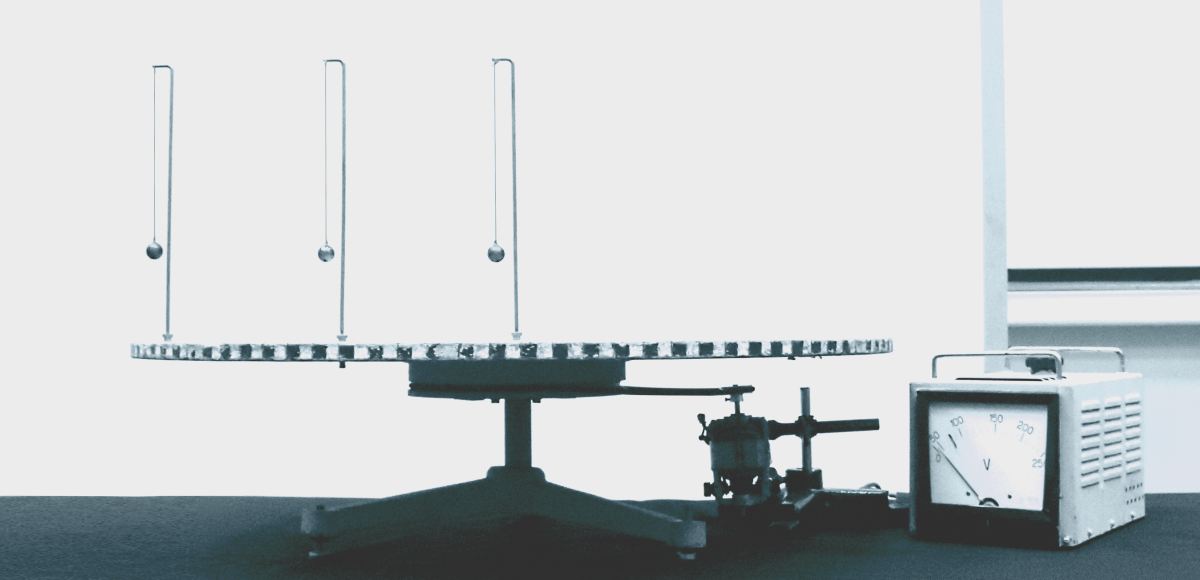
\includegraphics[width=0.9\linewidth]{platform-1.png}
		\caption{Демонстрация центробежной силы инерции}
		\label{platform-1}
	\end{figure}
	
	\subsection*{\underline{Оборудование:}}

	\begin{enumerate} 
		\item Шарики одинакового размера и массы, подвешенные на специальных стойках.
		\item Платформа с отверстиями для укрепления стоек с шариками.
		\item Электродвигатель с фрикционным индуктором.
		\item Вращающаяся подставка для платформы.
		\item Резиновое кольцо для передачи вращательного момента от вала двигателя к платформе.
		\item Лабораторный трансформатор (ЛАТР).
		\item Центробежная машина с червячной передачей.
	\end{enumerate}

	\subsection*{\underline{Основные определения:}}
		
		Центробежная сила инерции — псевдосила, действующая на материальную точку в неинерциальной системе отсчета, 
		направленная по главной нормали к ее траектории от центра кривизны 
		(от центра окружности при движении точки по окружности).
		Численно центробежная сила равна $ mv^2/l $, где \textit{m} — масса точки, \textit{v} — модуль ее линейной скорости, \textit{l} — радиус кривизны траектории.
		Под действием центробежной силы материальная точка движется криволинейно. 
		Поэтому при прямолинейном движении эта сила равна нулю.
		
		Нормальное ускорение является составляющей полного ускорения точки при криволинейном движении.
		Направлено такое ускорение по главной нормали к траектории в сторону центра кривизны.
		Обычно термин «нормальное ускорение» применяют в случае движения точки по окружности.
		
		Численно нормальная составляющая ускорения материальной точки равна $ v^2/l $, где \textit{v} — скорость точки, \textit{l} — радиус кривизны траектории.
		При движении по окружности нормальное ускорение может вычисляться по формуле $$ a = R\omega^2, $$ где \textit{R} — радиус окружности, $ \omega $ — угловая скорость вращения этого радиуса. 
		В случае прямолинейного движения нормальное ускорение также как и центробежная сила инерции обращается в нуль.

\subsection*{\underline{Краткое описание:}}
			
На вращающейся подставке укрепляют деревянный диск, вдоль радиуса которого на равных расстояниях друг от друга располагаются отвесы с металлическими шариками (рис.\ref{platform-2}).
Первый отвес находится на оси вращения диска, поэтому на него при вращении диска не действует центробежная сила инерции и шарик не отклоняется.

\begin{figure}[H] 
	\centering 		
	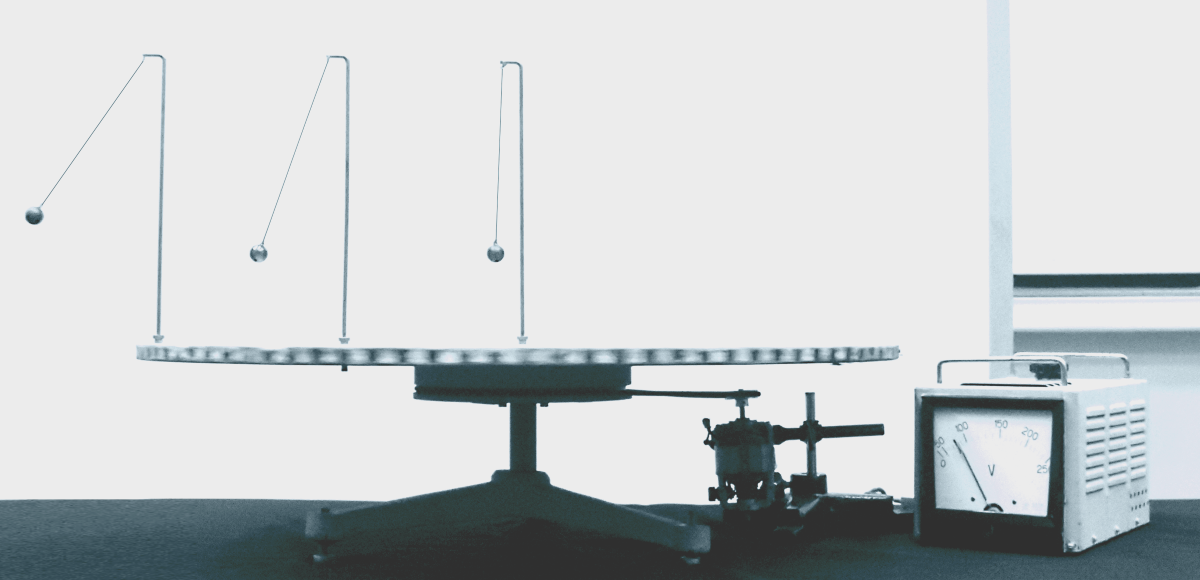
\includegraphics[width=0.8\linewidth]{platform-2.png} 
	\caption{Отклонение маятников от вертикали на вращающейся платформе. В зависимости от расстояния до оси вращения на одинаковые тела будут действовать различные силы инерции. О величине этих сил можно косвенно судить по величине угла отклонения каждого отвеса}
	\label{platform-2}
\end{figure}
	
На остальные отвесы действует центробежная сила инерции, пропорциональная расстоянию от оси вращения соответствующего отвеса.
Поэтому все шарики отклоняются на различные углы, тем больше, чем больше их расстояние от оси вращения.

\textit{Демонстрационные приборы на центробежной машине}. 
Центробежная машина служит для демонстрации опытов с физическими приборами:
\begin{enumerate} 
	\item \textit{Два тела неравной массы}. Прибор (рис.!!!!!) состоит из скобы, загнутые концы которой соединены стержнем. На стержень надеты два тела различной массы, соединенные между собой нитью. Скоба укреплена на конусном стержне, который служит для установки прибора в шпинделе центробежной машины. Такой же конусный стержень имеют все перечисленные ниже приборы.
	\item \textit{Регулятор центробежный}. Прибор (рис. \ref{regulator-1}) представляет собой два стержня с металлическими шарами на концах.
	Оба стержня подвижно укреплены к верхней части основного вертикального стержня. Эти стержни шарнирно связаны с тягами и с муфтой, скользящей по вертикальному стержню. Между верхней частью этого стержня и муфтой находится пружина, которая при подъеме муфты давит на нее и стремится поставить в исходное положение.
	При приведении в действие центробежной машины шары со стержнями в результате действия центробежной силы расходятся в стороны от вертикального стержня, а муфта поднимается вверх.
	\end{enumerate}

	% \textit{Сирена дисковая}. Сирена (рис.!!!!!) представляет собой металлический диск с четырьмя рядами отверстий числом: 48, 60, 72 и 96, расположенными по концентрическим окружностям. К прибору прилагается сопло с отверстием.
	%Дисковая сирена устанавливается в шпинделе центробежной машины, а сопло резиновой трубкой с нагнетательным воздушным насосом. Приводят в действие воздуходувку и одновременно равномерно вращают машину. Сопло подносят к какому-либо ряду отверстий сирены и получают звук одного тона. За неимением воздуходувки можно вместо сопла приложить к отверстиям сирены угол куска упругого картона или кусок листового целлулоида, что так же дает звук. 
	% В КОЛЕБАНИЯ Диск сирены может быть использован для демонстрации гармонического колебательного движения. Для этой цели в одном из отверстий диска устанавливают стержень с шариком (рис.). Центробежную машину с диском помещают на расстоянии 1 м от экрана. С противоположной стороны машины располагают источник света (около 2 м от машины). Источник света должен быть близок к точечному. При равномерном вращении диска сирены, тень шарика на экране будет совершать простое гармоническое движение.
	% В ОПТИКУ \textit{Круг Ньютона}. Прибор состоит из металлического диска, установленного на конусном стержне. На диске уложены семь бумажных полукруглов (красный, оранжевый, желтый, зеленый, голубой, синий и фиолетовый), котореы могут смещаться. Бумажные полукруги удерживаются на диске с помощью ранта по ободу и зажимной гайкой - в центре.
%Шпиндель центробежной машины устанавливают в горизонтальном положении (рис) и вставляют в него круг Ньютона с цветными секторами равной величины. При равномерном вращении машины вместо отдельных цветных секторов наблюдается однородный светлосерый  диск. Диск при этомдолжен быть хорошо освещен.

\textit{Опыт 1}. Два тела неравной массы, изготовленные в виде цилиндров, связанных нитью, раздвигают на 4-6 см один от другого и помещают на стержне так, чтобы расстояние их центров от оси вращения были приблизительно равными. При приведении машины во вращательное движение большой цилиндр перемещается к концу скобы и увлекает за собой малый. Если же расположить цилиндры от оси вращения на расстояния, обратно пропорциональные их массам, то во время вращения машины они останутся на своих местах.

\textit{Опыт 2}. В ходе демонстрации центробежного регулятора его вставляют в шпиндель машины.
При приведении машины во вращение наблюдают сжатие пружины вследствие подъема шариков вдоль вертикальной оси.

\begin{figure}[H] 
	\centering 		
	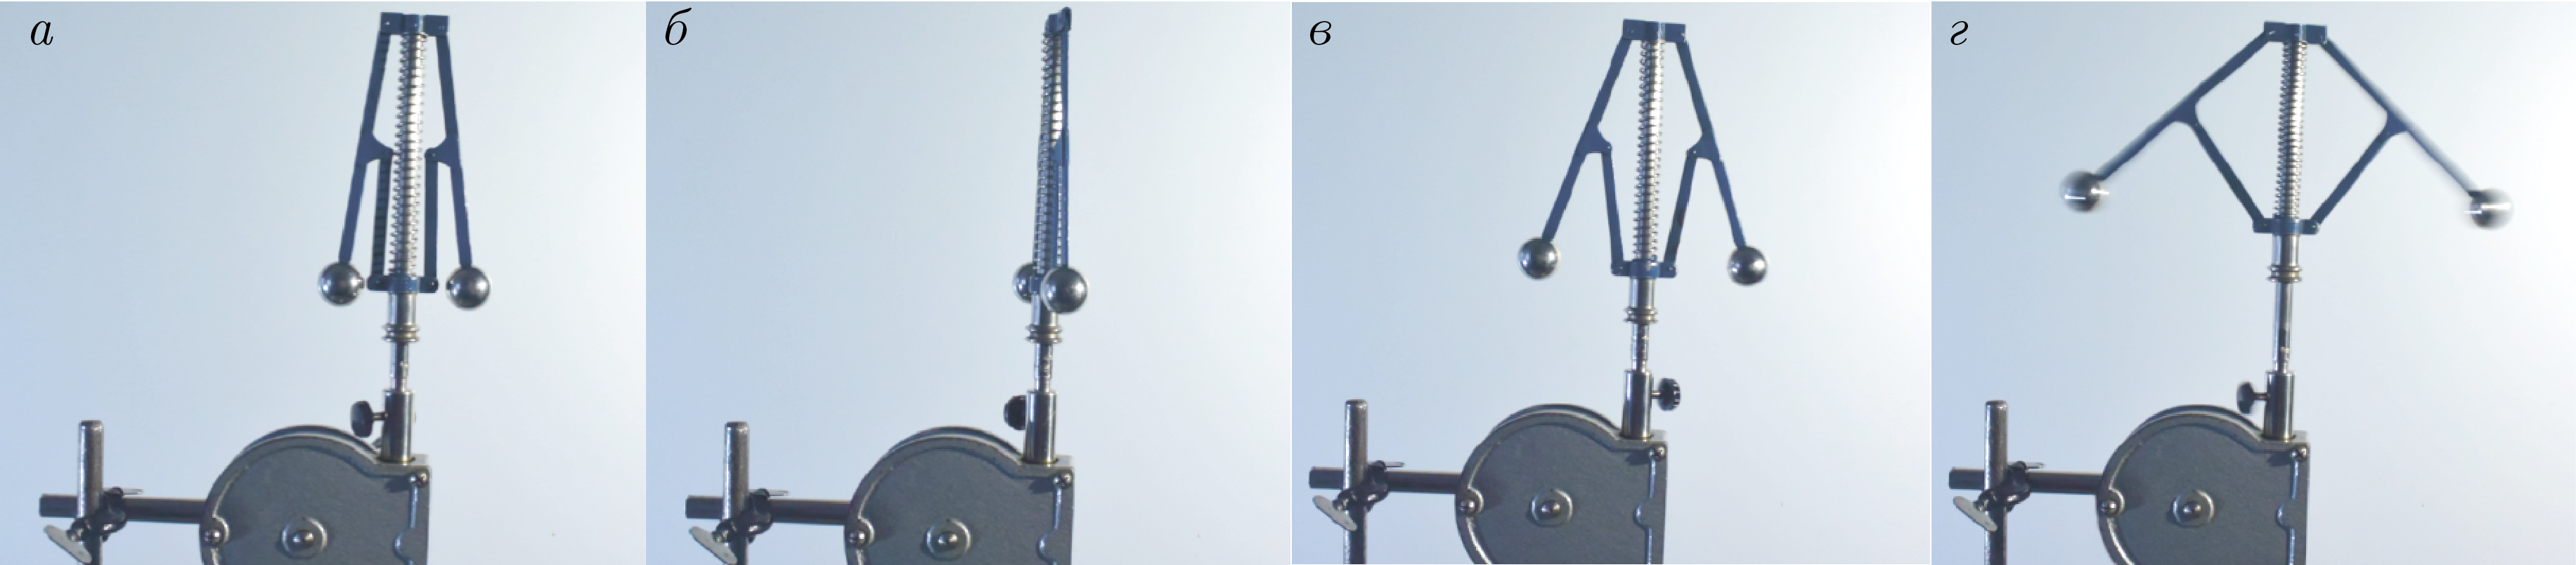
\includegraphics[width=0.9\linewidth]{regulator-1.png} 
	\caption{Возникающие при вращении центробежные силы инерции создают вращательный момент на стержни, и шары, поднимаясь в вертикальной плоскости, вызывают сжатие пружины регулятора}
	\label{regulator-1}
\end{figure}

\subsection*{\underline{Теория:}}

При вращении платформы с постоянной угловой скоростью $ \omega $ отвесы маятников отклоняются от вертикального положения, причем углы отклонения отвесов будут тем большие, чем дальше от центра платформы располагаются отвесы (рис.\ref{platform-3}).

\begin{figure}[H] 
	\centering 		
	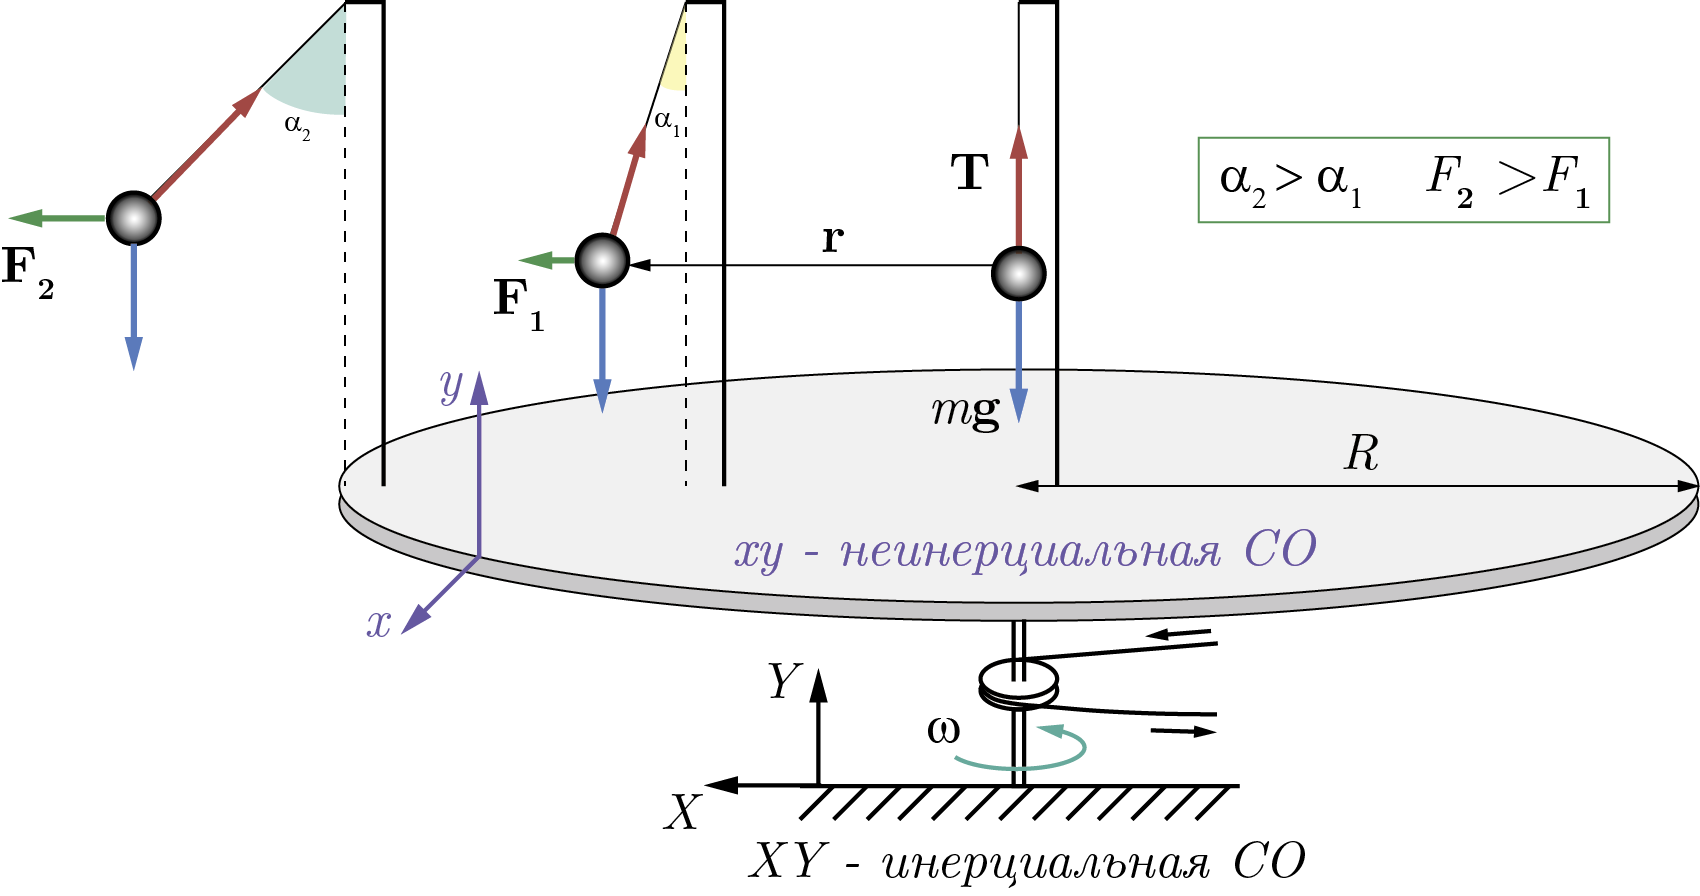
\includegraphics[width=0.9\linewidth]{platform-3.png} 
	\caption{Схематичное изображение поведения грузов на вращающейся платформе, расстояние от каждого из которых до оси вращения различается}
	\label{platform-3}
\end{figure}

Рассмотрим отклонения отвесов маятников относительно наблюдателя, находящегося в инерциальной
системе отсчета \textit{XY} (связана с Землей), и относительно наблюдателя, находящегося в неинерциальной вращающейся системе \textit{xy} (связана с вращающейся платформой). 



Относительно наблюдателя в ИСО отвесы отклоняются, а груз в этом случае находится под действием двух реальных сил: силы тяжести $ m\textbf{g} $ и силы натяжения нити $ \textbf{T} $.
Результирующая сила сообщает маятнику нормальное ускорение $ \textbf{a}_{\text{н}} = -\omega^{2}\textbf{r}  $, поэтому можно записать

\begin{equation}\label{platform-1eq1}
m\textbf{g}+\textbf{T}=-m\omega^{2}\textbf{r},
\end{equation}
где $ \textbf{r} $ — радиус-вектор, проведенный от оси вращения платформы до рассматриваемого груза.

Угол отклонения отвесов будет определяться соотношением:

\begin{equation}\label{platform-1eq2}
\text{tg} \alpha =\frac{m\omega^{2}r}{mg} = \frac{\omega^{2}r}{g}.
\end{equation}

Относительно наблюдателя, находящегося в НИСО (на подвижной платформе), при равномерной скорости вращения отвесы остаются в покое (неподвижны относительно наблюдателя).
Из этого следует, что сумма всех сил, действующих на груз $ m $, в этой системе отсчета должна обращаться в нуль.
Таким образом, наблюдатель, вращающийся вместе с грузами в системе отсчета \textit{xy} может сделать вывод, что на каждый маятник должна действовать некоторая сила, уравновешивающая известную пару реальных сил (притяжения и реакции со стороны подвеса).
Причем эта сила будет обязательно направлена из центра вдоль Вектора \textbf{r}. 
В качестве такой силы обычно рассматривается центробежная сила инерции \textbf{F} (рис.\ref{platform-3}), которая по своей природе является силой инерции.

Запишем уравнение движения маятника во вращающейся системе отсчета в векторной форме с учетом этой силы
\begin{equation}\label{platform-1eq3}
m\textbf{g}+\textbf{T}+\textbf{F}=0.
\end{equation}

Сравнивая его с выражением (\ref{platform-1eq1}), видим, что центробежная сила инерции может быть определена как $ \textbf{F}=m\omega^{2}\textbf{r} $.

Величина центробежной силы инерции, действующей на тела во вращающихся системах отсчета, зависит только от угловой скорости вращения $ \omega $ этой системы отсчета и от расстояния \textit{r} до оси вращения.
Важно, что она не зависит от скорости тел относительно вращающихся систем отсчета.
Иными словами, центробежная сила инерции действует во вращающихся системах отсчета на все без исключения материальные тела независимо от того, покоятся ли они в этих системах или движутся с некоторой относительной скоростью.
				
\end{document}
